\setcounter{section}{6}
\section{TP07 - Properties of regular languages}
{
\renewcommand{\thesubsubsection}{\thesubsection\alph{subsubsection}}
\begin{lemma}[Pumping lemma for REs] \label{lem:pump}
Given an infinite regular language $L \in \Sigma^*$,
\begin{equation*}
	\exists n \in \mathbb{N}^+ \colon \forall w, |w|\geq n \implies \exists x, y, z \in \Sigma^* \colon 
	\begin{cases}
		w = xyz \\
		|x\,y| \leq n\\
		|y| \geq 1\\
		\forall k \in \mathbb{N},\,x\,y^k\,z \in L
	\end{cases}
\end{equation*} 
\end{lemma}
\subsection{Exercise 1}
\subsubsection{Item a}
\begin{theorem}
	$L=\{0^n1^{2n}\;|\;n\geq 1\}$ is not a regular language.
\end{theorem}
\begin{proof}
Assume by absurd that $L$ is a regular language. Then by the pumping lemma \eqref{lem:pump},
\begin{equation*}
	\exists n \in \mathbb{N}^+ \colon \forall w, |w|\geq n \implies \exists x, y, z \in \Sigma^* \colon 
	\begin{cases}
		w = xyz \\
		|x\,y| \leq n\\
		|y| \geq 1\\
		\forall k \in \mathbb{N},\,x\,y^k\,z \in L
\end{cases}
\end{equation*}
Say we know the value of $n$. Now consider the string $w=0^n1^{2n}$, that verifies $|w|=3n \geq n$. So we know that
\begin{equation*}
\exists x, y, z \in \Sigma^* \colon 
\begin{cases}
	w = xyz \\
	|x\,y| \leq n\\
	|y| \geq 1\\
	\forall k \in \mathbb{N},\,x\,y^k\,z \in L
\end{cases}
\end{equation*}
Then, $x$, $y$ and $z$ must be of the form
\begin{alignat*}{2}
	x &= 0^a\\
	y &= 0^b\\
	z &= 0^c1^{2n}
\end{alignat*}
where $b \geq 1$, $a+b \leq n$ and $c=n-a-b$.\\
Say these strings $x$, $y$ and $z$ are the ones that obey the pumping lemma. Then we have that
\begin{equation*}
	\forall k \in \mathbb{N},\,x\,y^k\,z \in L
\end{equation*}
So, let's instantiate to $k=2$.
\begin{alignat*}{2}
	x\,y^2\,z \in L
	& \iff \exists m \geq 1 \colon x\,y^2\,z           &&= 0^m1^{2m} \\
	& \iff \exists m \geq 1 \colon 0^a(0^b)^20^c1^{2n} &&= 0^m1^{2m} \\
	& \iff \exists m \geq 1 \colon 0^{a+2b+c}1^{2n}    &&= 0^m1^{2m} \\
	& \iff \exists m \geq 1 \colon 0^{a+b+c+b}1^{2n}   &&= 0^m1^{2m} \\
	& \iff \exists m \geq 1 \colon 0^{n+b}1^{2n}       &&= 0^m1^{2m} \\
	& \iff 2(n+b)                                      &&= 2n\\
	& \iff n+b                                         &&= n\\
	& \iff b                                           &&= 0
\end{alignat*}
which is trivially false given that $b \geq 1$. Now all that is left to do is conclude the contradiction will propagate all the way up the proof, thus proving the theorem correct.
\end{proof}
\pagebreak
\subsubsection{Item b}
\begin{theorem}
$L=\{v1^{|v|}\,|\,v \in \{0,1\}^*\}$ is not a regular language.
\end{theorem}
\begin{proof}
Assume  by absurd that $L$ is a regular language. The by the pumping lemma \eqref{lem:pump},
\begin{equation*}
	\exists n \in \mathbb{N}^+ \colon \forall w, |w|\geq n \implies \exists x, y, z \in \Sigma^* \colon 
	\begin{cases}
		w = xyz \\
		|x\,y| \leq n\\
		|y| \geq 1\\
		\forall k \in \mathbb{N},\,x\,y^k\,z \in L
\end{cases}
\end{equation*}
Say we know the value of $n$. Now consider the string $w=0^n1^n$, that verifies $|w|=2n \geq n$. So we know that
\begin{equation*}
\exists x, y, z \in \Sigma^* \colon 
\begin{cases}
	w = xyz \\
	|x\,y| \leq n\\
	|y| \geq 1\\
	\forall k \in \mathbb{N},\,x\,y^k\,z \in L
\end{cases}
\end{equation*}
Then, $x$, $y$ and $z$ must be of the form
\begin{alignat*}{2}
	x &= 0^a\\
	y &= 0^b\\
	z &= 0^c1^{n}
\end{alignat*}
where $b \geq 1$, $a+b \leq n$ and $c=n-a-b$.\\
Say these strings $x$, $y$ and $z$ are the ones that obey the pumping lemma. Then we have that
\begin{equation*}
	\forall k \in \mathbb{N},\,x\,y^k\,z \in L
\end{equation*}
So, let's instantiate to $k=2$.
\begin{alignat*}{2}
	x\,y^2\,z \in L
	& \iff 0^a(0^b)^20^c1^n &&\in L \\
	& \iff 0^{a+2b+c}1^n    &&\in L \\
	& \iff 0^{a+b+c+b}1^n   &&\in L \\
	& \iff 0^{n+b}1^n       &&\in L
\end{alignat*}
It is both trivial that $|v 1^{|v|} | = 2|v|$ and that $|w|=|0^{n+b}1^n|=2n+b$.\\
This means that if $|w| \equiv 1 \pmod{2}$ then this system is false.\\
If $|w| \equiv 0 \pmod{2}$, then for $w$ to belong to $L$ it would be necessary to check that the last $|w|/2$ symbols are all $1$. This is not the case, because the last $|w|/2$ symbols are $0^{|w|/2-n}1^n$ and $|w|/2-n > 0$ (given that $|w|=2n+b \iff |w|/2=n+b/2 \iff |w|/2-n=b/2$ and $b \geq 1$).\\
Now all that is left to do is conclude the contradiction will propagate all the way up the proof, thus proving the theorem correct.
\end{proof}
\subsubsection{Item c}
If the language can be represented by a RE, then it is regular. Thus, the language of the strings given by $(00+11)^*$ is trivially regular.
\subsubsection{Item d}
Idem.
\subsubsection{Item e}
\begin{theorem}
$L=\{0^n\,|\,n \text{ is a perfect square}\}$ is not a regular language.
\end{theorem}
\begin{proof}
Assume  by absurd that $L$ is a regular language. The by the pumping lemma \eqref{lem:pump},
\begin{equation*}
	\exists n \in \mathbb{N}^+ \colon \forall w, |w|\geq n \implies \exists x, y, z \in \Sigma^* \colon 
	\begin{cases}
		w = xyz \\
		|x\,y| \leq n\\
		|y| \geq 1\\
		\forall k \in \mathbb{N},\,x\,y^k\,z \in L
\end{cases}
\end{equation*}
Say we know the value of $n$. Now consider the string $w=0^n$ where $n$ is a perfect square, that verifies $|w|=n \geq n$. So we know that
\begin{equation*}
\exists x, y, z \in \Sigma^* \colon 
\begin{cases}
	w = xyz \\
	|x\,y| \leq n\\
	|y| \geq 1\\
	\forall k \in \mathbb{N},\,x\,y^k\,z \in L
\end{cases}
\end{equation*}
Then, $x$, $y$ and $z$ must be of the form
\begin{alignat*}{2}
	x &= 0^a\\
	y &= 0^b\\
	z &= 0^c
\end{alignat*}
where $b \geq 1$, $a+b \leq n$ and $c=n-a-b$.\\
Say these strings $x$, $y$ and $z$ are the ones that obey the pumping lemma. Then we have that
\begin{alignat*}{2}
	\forall k \in \mathbb{N},\,x\,y^k\,z \in L
	& \iff \forall k \in \mathbb{N},\,0^a(0^b)^k0^c && \in L \\
	& \iff \forall k \in \mathbb{N},\,0^{a+kb+c}    && \in L \\
	& \iff \forall k \in \mathbb{N},\,0^{n+b(k-1)}  && \in L \\
	& \iff \forall k \in \mathbb{N},\,n+b(k-1)      && \text{ is a perfect square}
\end{alignat*}
This means the pumping lemma implies there are at least $\left\lfloor \frac{x-n}{b} \right\rfloor +1$ perfect squares less or equal to $x$.\\
There are exactly $\lfloor \sqrt{x} \rfloor +1$ perfect squares less or equal to $x$.\\
We will now proceed to find a definition of $x$ so as to arrive at the contradiction that the pumping lemma states there are more solutions than there can actually be.\\
Let us define $x=n\,f^2$. Now we have to find a function $f(n,b)$ such that
\begin{equation*}
	\left\lfloor \frac{n\,f^2-n}{b} \right\rfloor +1 > \lfloor \sqrt{n\,f^2} \rfloor +1
\end{equation*}
\begin{alignat*}{2}
	\left\lfloor \frac{n\,f^2-n}{b} \right\rfloor +1 > \lfloor \sqrt{n\,f^2} \rfloor +1
	&\iff \frac{n\,f^2-n}{b}+1 \geq \sqrt{n\,f^2} +2 \\
	&\iff \frac{n}{b}(f^2-1) \geq \sqrt{n}f + 1
\end{alignat*}
Given $b \leq n \iff n/b \geq 1$, the situation that makes the previous equation harder to be true is $n/b=1$.
\begin{alignat*}{2}
	f^2-1 \geq \sqrt{n}f + 1
	&\iff f^2-\sqrt{n}f-2 \geq 0
\end{alignat*}
The left-hand side of the inequality describes a parabola facing upwards and intersecting the $x$-axis, thus we are interested in a solution for $f$ to the right of the larger root.
 \begin{alignat*}{2}
	f^2-\sqrt{n}f-2 = 0
	&\iff f = \frac{\sqrt{n}+\sqrt{n+8}}{2}
\end{alignat*}
So, a function $f(n,b)=\sqrt{n+8}$ would perfectly fit its purpose.\\
Given we found such a function $f$, we have found a definition of $x$ that creates a contradiction. Now all that is left to do is conclude the contradiction will propagate all the way up the proof, thus proving the theorem correct.
\end{proof}
\subsection{Exercise 2}
\subsubsection{Item a}
\begin{theorem}
If $L$ is regular then $L/a$ is regular.
\end{theorem}
\begin{proof}
If $L$ is regular, it can be represented by a DFA. Let us call it $D$. We will prove this theorem by describing an algorithm to obtain the DFA of $L/a$, $D'$, from $D$.
\begin{enumerate}
	\item For each final state $q$:
	\begin{enumerate}
		\item If there is a transition $r \xrightarrow{s} q$ then there is a transition $r \xrightarrow{s} q_s$
		\item If there is a transition $q \xrightarrow{a} r$ then there is a transition $q_s \xrightarrow{a} r$ 
	\end{enumerate}
	This DFA is equivalent to $D$, but each final state has only inward transitions from a sigle symbol $s$.
	\item Mark each final state $q_s$ with $s \neq a$ as non-final states.\\
	This DFA is equivalent to $D$, except it rejects all strings that do not end in $a$.
	\item For each final state $q$, mark all states from which $q$ can be reached as final states, and mark $q$ as non-final.\\
	This DFA accepts all strings that the previous DFA accepted, but without the need to have the $a$ at the end.
\end{enumerate}
This is exactly the algorithm we wanted to design. We have thus proven the theorem correct.
\end{proof}
\subsubsection{Item b}
\begin{theorem}
If $L$ is regular then $a\backslash L$ is regular.
\end{theorem}
\begin{proof}
It is trivial that $a \backslash L=(L^{-1}/a)^{-1}$. Given that regular languages are closed to the reverse $^{-1}$ and the quotient $/$ operations, $L^{-1}$, $L^{-1}/a$ and $(L^{-1}/a)^{-1}$ are all regular languages, thus making $a \backslash L$ a regular language.
\end{proof}
\subsubsection{Item c}
\begin{itemize}
	\item False. $L=\{b\}$, $L/a=\emptyset$, $(L/a)a=\emptyset$.
	\item False. $L=\{b\}$, $a \backslash L = \emptyset$, $a(a \backslash L)=\emptyset$.
	\item True.
	\item True.
\end{itemize}
\subsection{Exercise 3}
\begin{theorem}
Given $L_2=\{0^n1^n\,|\,n \geq 0\}$ is not a regular language, $L_1=\{0^i1^j\,|\,i \neq j\}$ is not a regular language.
\end{theorem}
\begin{proof}
$L_2=\overline{L_1} \cap L(0^*1^*)$. Assuming $L_1$ is regular, and given regular languages are closed to negation $\overline{L}$ and intersection $\cap$, and since $L(0^*1^*)$ is regular, then $L_2$ is also regular. The theorem we want to prove is the contrapositive of what was just said, so the theorem is thus proven correct.
\end{proof}
\subsection{Exercise 4}
\subsubsection{Item a}
Consider all strings $w \in \Sigma^*$ such that $n \leq |w| < 2n$ where $n$ is the number of states of the DFA, and test each of them for acceptance by the DFA. If one of them is accepted, then it means there is a loop in the DFA, because a loopless DFA would not be able to recognize a string with at least $n$ symbols without having at least $n+1$ states. String $w=x\,y^2\,z$ getting accepted means the string took string $x$ to reach the loop, went around the loop twice, each time using string $y$, and then took string $z$ to reach an accept state. This implies any string of the form $x\,y^k\,z$ is accepted by the language, thus making it infinite.
\subsubsection{Item b}
Consider the negated DFA, and check if the corresponding language is empty by testing if any string $w \in \Sigma^*$ such that $0 \leq |w| < n$ (where $n$ is the number of states of the DFA) is accepted.
\subsection{Exercise 5}
\subsubsection{Item a}
First step: if $p$ is final and $q$ is not, $(p,q)$ are distinguishable.
\begin{center} \begin{tabular}{r || c | c | c | c | c | c | c | c | c}
	   & A  & B  & $^*$C & D  & E  & $^*$F & G  & H  & $^*$I \\ \hline \hline
	A  & \cellcolor{gray} & \cellcolor{gray} & \cellcolor{gray} & \cellcolor{gray} & \cellcolor{gray} & \cellcolor{gray} & \cellcolor{gray} & \cellcolor{gray} & \cellcolor{gray} \\ \hline
	B  &    & \cellcolor{gray} & \cellcolor{gray} & \cellcolor{gray} & \cellcolor{gray} & \cellcolor{gray} & \cellcolor{gray} & \cellcolor{gray} & \cellcolor{gray} \\ \hline
	$^*$C & X  & X  & \cellcolor{gray} & \cellcolor{gray} & \cellcolor{gray} & \cellcolor{gray} & \cellcolor{gray} & \cellcolor{gray} & \cellcolor{gray} \\ \hline
	D  &    &    & X  & \cellcolor{gray} & \cellcolor{gray} & \cellcolor{gray} & \cellcolor{gray} & \cellcolor{gray} & \cellcolor{gray} \\ \hline
	E  &    &    & X  &    & \cellcolor{gray} & \cellcolor{gray} & \cellcolor{gray} & \cellcolor{gray} & \cellcolor{gray} \\ \hline
	$^*$F & X  & X  &    & X  & X  & \cellcolor{gray} & \cellcolor{gray} & \cellcolor{gray} & \cellcolor{gray} \\ \hline
	G  &    &    & X  &    &    & X  & \cellcolor{gray} & \cellcolor{gray} & \cellcolor{gray} \\ \hline
	H  &    &    & X  &    &    & X  &    & \cellcolor{gray} & \cellcolor{gray} \\ \hline
	$^*$I & X  & X  &    & X  & X  &    & X  & X  & \cellcolor{gray} 
\end{tabular} \end{center}
Second step: repeat while there are changes; if $\delta(p,a)$ and $\delta(q,a)$ are distinguishable, then $(p,q)$ are distinguishable.
\begin{center} \begin{tabular}{r || c | c | c | c | c | c | c | c | c}
	   & A  & B  & $^*$C & D  & E  & $^*$F & G  & H  & $^*$I \\ \hline \hline
	A  & \cellcolor{gray} & \cellcolor{gray} & \cellcolor{gray} & \cellcolor{gray} & \cellcolor{gray} & \cellcolor{gray} & \cellcolor{gray} & \cellcolor{gray} & \cellcolor{gray} \\ \hline
	B  & X  & \cellcolor{gray} & \cellcolor{gray} & \cellcolor{gray} & \cellcolor{gray} & \cellcolor{gray} & \cellcolor{gray} & \cellcolor{gray} & \cellcolor{gray} \\ \hline
	$^*$C & X  & X  & \cellcolor{gray} & \cellcolor{gray} & \cellcolor{gray} & \cellcolor{gray} & \cellcolor{gray} & \cellcolor{gray} & \cellcolor{gray} \\ \hline
	D  &    & X  & X  & \cellcolor{gray} & \cellcolor{gray} & \cellcolor{gray} & \cellcolor{gray} & \cellcolor{gray} & \cellcolor{gray} \\ \hline
	E  & X  &    & X  & X  & \cellcolor{gray} & \cellcolor{gray} & \cellcolor{gray} & \cellcolor{gray} & \cellcolor{gray} \\ \hline
	$^*$F & X  & X  &    & X  & X  & \cellcolor{gray} & \cellcolor{gray} & \cellcolor{gray} & \cellcolor{gray} \\ \hline
	G  &    & X  & X  &    & X  & X  & \cellcolor{gray} & \cellcolor{gray} & \cellcolor{gray} \\ \hline
	H  & X  &    & X  & X  &    & X  & X  & \cellcolor{gray} & \cellcolor{gray} \\ \hline
	$^*$I & X  & X  &    & X  & X  &    & X  & X  & \cellcolor{gray} 
\end{tabular} \end{center}
\subsubsection{Item b}
\begin{center}
\begin{minipage}[c]{0.45\textwidth}
\begin{center} \begin{tabular}{r | c c}
	$\delta   $ & $0        $ & $1        $ \\ \hline
	$\{A,D,G\}$ & $\{B,E,H\}$ & $\{B,E,H\}$ \\
	$\{B,E,H\}$ & $\{C,F,I\}$ & $\{C,F,I\}$ \\
	$\{C,F,I\}$ & $\{A,D,G\}$ & $\{B,E,H\}$
\end{tabular} \end{center}
\end{minipage}%
\begin{minipage}[c]{0.25\textwidth}
\begin{center} 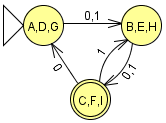
\includegraphics[scale=0.5]{TP07_5b} \end{center}
\end{minipage}
\end{center}
\subsection{Exercise 6}
\subsubsection{Item a}
\begin{center} \begin{tabular}{r | c c}
	$\delta$ & $a$ & $b$ \\ \hline
	$\rightarrow^*$A  & B  & E  \\
	$^*$B  & B  & C  \\
	$^*$C  & D  & C  \\
	D      & D  & D  \\
	$^*$E  & D  & E  
\end{tabular} \end{center}
\begin{center} \begin{tabular}{r || c | c | c | c | c}
	       & $^*$A  & $^*$B  & $^*$C & D  & $^*$E  \\ \hline \hline
	$^*$A  & \cellcolor{gray} & \cellcolor{gray} & \cellcolor{gray} & \cellcolor{gray} & \cellcolor{gray} \\ \hline
	$^*$B  &    & \cellcolor{gray} & \cellcolor{gray} & \cellcolor{gray} & \cellcolor{gray} \\ \hline
	$^*$C  &    &    & \cellcolor{gray} & \cellcolor{gray} & \cellcolor{gray} \\ \hline
	D      & X  & X  & X  & \cellcolor{gray} & \cellcolor{gray} \\ \hline
	$^*$E  &    &    &    & X  & \cellcolor{gray}
\end{tabular} \end{center}
\begin{center} \begin{tabular}{r || c | c | c | c | c}
	       & $^*$A  & $^*$B  & $^*$C & D  & $^*$E  \\ \hline \hline
	$^*$A  & \cellcolor{gray} & \cellcolor{gray} & \cellcolor{gray} & \cellcolor{gray} & \cellcolor{gray} \\ \hline
	$^*$B  &    & \cellcolor{gray} & \cellcolor{gray} & \cellcolor{gray} & \cellcolor{gray} \\ \hline
	$^*$C  & X  & X  & \cellcolor{gray} & \cellcolor{gray} & \cellcolor{gray} \\ \hline
	D      & X  & X  & X  & \cellcolor{gray} & \cellcolor{gray} \\ \hline
	$^*$E  & X  & X  &    & X  & \cellcolor{gray}
\end{tabular} \end{center}
\begin{center}
\begin{minipage}[c]{0.40\textwidth}
\begin{center} \begin{tabular}{r | c c}
	$\delta                $ & $a      $ & $b      $ \\ \hline
	$\rightarrow ^* \{A,B\}$ & $\{A,B\}$ & $\{C,E\}$ \\
	$            ^* \{C,E\}$ & $\{D  \}$ & $\{C,E\}$ \\
	$               \{D  \}$ & $\{D  \}$ & $\{D  \}$
\end{tabular} \end{center}
\end{minipage}%
\begin{minipage}[c]{0.35\textwidth}
\begin{center} 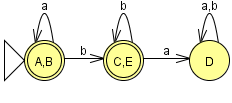
\includegraphics[scale=0.5]{TP07_6a} \end{center}
\end{minipage}
\end{center}
\subsubsection{Item b}
The automata $FA_1$ and $FA_2$ are equivalent, given the only difference between them is the names of the states.
}
